\documentclass[11pt]{article}
\usepackage[utf8]{inputenc}
\usepackage[T1]{fontenc}
\usepackage{amsmath}
\usepackage{amsfonts}
\usepackage{amssymb}
\usepackage[version=4]{mhchem}
\usepackage{stmaryrd}
\usepackage{graphicx}
\usepackage[export]{adjustbox}
\graphicspath{ {./images/} }

\begin{document}
Infrastructure

In finance, infrastructure refers to the underlying and fundamental assets and systems that facilitate functions that are necessary to the well-being of an economy. Not all infrastructure assets are conducive to being privately financed. Infrastructure assets are a means for ensuring the delivery of goods and services that promote prosperity and growth and contribute to quality of life, including the social well-being, health, and safety of citizens and the quality of their environments. For example, it may be argued that agricultural ventures are part of infrastructure in view of their being essential to the economy and population of a country. However, in most economies, agricultural assets are privately financed.

\section*{Seven Elements That Help Identify Investable Infrastructure}
Defining investable infrastructure is challenging. Some market participants define investable infrastructure based on having risks and returns that are distinct from those of traditional investments and that require specialized tools of analysis. Other market participants focus on the extent to which the investments are financial claims on infrastructure assets. For our purposes, investable infrastructure is typically differentiated from other assets with seven primary characteristics: (1) public use, (2) monopolistic power, (3) government related, (4) essential, (5) cash generating, (6) conducive to privatization of control, and (7) capital intensive with longterm horizons.

\begin{enumerate}
  \item Public use refers to the idea that the associated economic activity is accessed by a large segment of the population or is viewed as serving the general welfare of a society.

  \item Monopolistic power refers to the extent to which services are offered by a single provider or are offered such that the provider can set prices relatively free from competition.

  \item Government related refers to the extent to which the underlying assets are typically created by, owned by, managed by, or heavily regulated by government.

  \item Infrastructure assets tend to provide essential goods or services, such as electricity distribution. Hence, the demand for the goods or services is usually price inelastic, and cash inflows tend to be stable and inflation-protected.

  \item Investable infrastructure tends to be focused on assets that directly generate cash, such as toll roads, rather than similar assets that are supported by general tax revenues, such as highways other than toll roads.

  \item Investable infrastructure may possess attributes that make the underlying assets and systems relatively conducive to privatization of managerial control.

  \item Investable infrastructure is usually capital intensive, with underlying assets that are long-term in nature.

\end{enumerate}

To the extent that these elements are satisfied, an asset is more likely to be considered an investable infrastructure asset. However, no single element is necessary or sufficient. For example, a municipal bond backed by revenues from a toll road would generally not be considered investable infrastructure even though it may satisfy almost all of the aspects found in investable infrastructure discussed here. In the case of a municipal bond, there is no privatization of the toll road or change in managerial control if the toll road remains under the full authority of a governmental organization. The equity of a firm that manufactures a common and essential vaccine may satisfy all of the listed aspects of investable infrastructure except that such equity is not traditionally governmentally owned. Fortunately, the major types of investable infrastructure are reasonably well defined, as shown in the next exhibit, Infrastructure Investment Universe.

Infrastructure Investment Universe

\begin{center}
\begin{tabular}{|lc|}
\hline
Economic Infrastructure & Social Infrastructure \\
\hline
Transport & Education facilities \\
Toll roads, bridges, tunnels & Schools \\
Airports & Universities \\
Seaports & Health-care facilities \\
Rail networks & Hospitals \\
Utilities & Aged care \\
Distribution of gas, electricity, and other energy sources & Child care \\
Treatment and distribution of water & Correctional facilities \\
Renewable energy & Courts \\
Communications infrastructure & Jails, prisons \\
Specialty sectors &  \\
Car parks &  \\
Storage facilities &  \\
Forests &  \\
\end{tabular}
\end{center}

Source: Asieh Mansour and Hope Nadji, “Opportunities in Private Infrastructure Investments in the U.S.," RREEF Research, September 2006.

Investable infrastructure can originate as a new, yet-to-be-constructed project, referred to as a greenfield project, that was designed to be investable. Investable infrastructure can also be an existing project, or brownfield project, that has a history of operations and may have converted from a government asset into something privately investable. New projects may be funded by private capital rather than through government control and financing in order to promote efficiency and enable construction without straining government resources. Existing projects are converted to investable infrastructure primarily to raise capital for government and to earn cash flow for private investors.

The critical property of infrastructure (i.e., the most important distinction between investable infrastructure and traditional investments) is in the nature of the revenues, with investable infrastructure generating a cash flow stream in a monopolistic environment rather than in a competitive environment. An investment in\\
infrastructure generally relies on the purchase or long-term lease of a facility that generates stable cash flows, ideally growing with the rate of inflation.

\section*{Economic versus Social Infrastructure}
As shown in the exhibit above infrastructure investments can be divided into the two broad categories of economic and social infrastructure. Economic infrastructure assets are assets with economic value that is driven by the revenue they generate, typically with end users paying for the services provided by these assets. Examples of these are toll roads and bridges, railways, airports, and maritime terminals. Social infrastructure assets are assets that have end users who are unable to pay for the services or that are used in such a way that it is difficult to determine how many services were used by each person; examples include schools, public roads, prisons, administrative offices, and other government buildings.

Notice how these infrastructure categories fit the previous discussion, as transportation or utility assets often have the characteristics of a natural or regulated monopoly, in which users have a low price elasticity of demand. When necessary services are provided, users do not typically reduce their usage substantially as a result of price increases; this means that the service providers have pricing power, which allows price increases to result in revenue increases.

Infrastructure assets can be categorized according to who the payer is, with a distinction that is similar to the difference between economic and social infrastructure. Often the end user pays to use the assets. Examples of these are toll roads, utilities, and communications networks. Government and taxpayers pay for the use of assets. In this case, the asset is mostly or partially free for the end users. Examples of these are many schools and some hospitals, administrative buildings, and parks.

\section*{Public-Private Partnerships in Infrastructure Investing}
Governments have long recognized that investments in infrastructure produce positive externalities, contribute to economic growth, expand market access, and reduce inefficiencies. From a public policy perspective, improvements in regulation, governance, transparency, ethics, property rights, and external checks are necessary and go a long way in encouraging private-sector participation in infrastructure projects. Given the extremely high up-front capital costs in establishing projects, infrastructure assets exhibit natural monopoly characteristics; often a single firm can produce essential social service outputs at greater efficiencies and at lower social costs than can multiple competitive firms. Recognizing this, governments restrict competition and create statutory monopolies.

Many existing infrastructure assets were built with public funds and then sold into the private sector. When a governmental entity sells a public asset to a private operator, this is termed privatization. While some argue that the private sector operates assets more efficiently, others argue that privatization is unfair to publicsector workers or otherwise contrary to the public interest. Although many privatizations take the form of the outright sale of an asset, in other cases, the governmental entity retains a stake in the asset. A public-private partnership (PPP) is a collaboration between public bodies, governments, and the private sector that occurs when a private-sector party is retained to design, build, operate, or maintain a public building (e.g., a hospital), for a lease payment with a finite time. Popular are leases or concessions wherein the government leases an asset to a private operator for 20 to 99 years, with the full equity interest in the facility reverting to public ownership at the end of the concession term. The partnerships extend across a variety of sectors, which can include transportation, water supply, and waste management, as well as the building and managing of hospitals, schools, public housing, and prisons. PPPs can take a wide variety of forms, with varying involvement of the private sector and varying degrees of risk transfer from government to the private sector.

PPPs and regulated assets (as in economic regulation, with the regulator setting prices) are normally mutually exclusive. A PPP is a finite concession with a price mechanism agreed to contractually up front. Privatized assets are owned by the private sector under a license, and prices are periodically set (or at least reviewed) by a regulator to ensure that they are appropriate and fair to the owner and to customers.

In order to enter into a greenfield PPP contract to design, build, operate, and own an infrastructure asset under a long-term government concession, private-sector investors form a special purpose vehicle (SPV) to act as concessionaire. Based on the concession contract and projected revenues from usage fees, the SPV receives equity capital from investors and enters into a contract with a design and construction company to build the asset. It may also enter into a separate contract with an operating company for the operation and maintenance of the infrastructure asset. The SPV also raises debt that can range from $60 \%$ to $90 \%$ of total project costs. Upon completion and commissioning of the infrastructure asset, the revenue generated through usage fees after payment of the concessionaire at the agreed-upon tariff rate is used to partly pay down debt, with the surplus passed on to equity contributors.

PPPs have faced opposition from advocacy groups and, sometimes, from the public. Criticism often takes the form of allegations of reduced accountability and the profit motive of the private sector, which may be at odds with the public interest. This criticism tends to be more intense in projects in which fees charged to the public are highly visible, such as in the case of toll roads. There have also been instances (although rare) of privatization reversals in response to allegations of underinvestment and poor asset upkeep. Many issues are driven by public perception. For example, municipalities may be reticent to declare future toll increases and may have minimal incentives to publish aggressive projections, for these can be politically unpalatable. Private concessionaires, in contrast, are less reluctant to establish explicit future increases.

Ideally, regulatory public policy with respect to PPPs would be consistent with technological innovation, capital needs, market developments, public opinion, and changing needs to create a balance between the multiple and often opposing constituencies. Issues that inevitably feature in policy discussions relate to economic transfers and distributional effects: for example, who benefits and at what cost to others, rents, accountability, regional development, jobs, prices, and tariffs. To preclude excess rent-seeking monopolistic behavior, infrastructure services may be procured under PPP with an agreed-upon pricing mechanism or may be heavily regulated. In some cases, regulation has not kept pace with the swift pace of innovation in this arena.

The degree of private investment within infrastructure depends on the commercial viability of the sector or subsector, as well as the governmental policy within a given country. Private-sector participation in economic infrastructure relies on a government that is content with essential assets being operated by the private sector, which charges citizens for its services (often within a regulated pricing structure). It also relies on customers' propensity to pay. For example, toll roads have been historically unpopular with many electorates; consequently, new roads are often procured as "shadow toll" PPPs, meaning that motorists do not pay the tolls. In developing countries, users may be unable to pay, resulting in the need for government support. Private investment in social infrastructure depends both on the government's ability to pay the private sector for the service and on the government's political support for the PPP.

\section*{Risks and Government Regulation of Infrastructure Investing}
Investors in infrastructure need to be keenly aware of governmental issues related to their investments, which can be either positive or negative. The scope and quality of a nation's infrastructure can influence its economic growth, with weaker infrastructure often blamed for reducing the economic growth potential of a\\
nation. One positive aspect of governmental issues on the infrastructure sector is the vast need for new or improved infrastructure assets combined with the constrained fiscal budgets of governments. In developed economies, infrastructure is aging and needs to be repaired, replaced, or improved. In developing economies, especially those with rapid population and income growth, there is a substantial demand for the creation of new infrastructure. In most countries, the scale of infrastructure needs far outstrips the ability of the government to fund the investment. Governments can use the proceeds from infrastructure leases or sales to fund other infrastructure projects or divert them to other fiscal needs. However, some governmental entities use those proceeds for spending or debt reduction, neither of which directly and immediately enhances the quality or availability of the infrastructure in an economy.

The revenues of infrastructure are closely linked to the prices of the services provided-which in turn is driven by the degree of pricing regulation. Regulated pricing occurs in most countries and the pricing for goods and services deemed essential is largely determined by price changes that must be approved by public entities and are most common in the energy sector. There is a growing trend toward unregulated pricing of certain infrastructure investments in mature countries.

There can be regulatory risk in a transaction. Regulatory risk is the economic dispersion to an investor from uncertainty regarding governmental regulatory actions and includes uncertain regulation regarding the initiation of a project or its operation. In some circumstances, a sale to investors may need to be approved by voters or a governing body, and therefore the consummation of a purchase is uncertain until all approvals have been obtained. Even after the completion of a purchase, investors in many infrastructure assets continue to find operations being regulated. Governmental entities, especially in the transport or utility sectors, are often involved in monitoring service quality and regulating prices or profit margins. Although regulating prices or margins may reduce profit potential, the right to run a monopoly business often leads to relatively stable cash flows. When assets are leased, the governmental entity may retain the right to revoke the lease if the service and maintenance of the assets do not meet the stated standards.

One example of regulatory risk can be seen in the case of Gassco, a joint venture between the Norwegian government and a number of large institutional investors that operated pipelines that delivered Norwegian natural gas to continental Europe. After 10 years of stable tariffs that allowed investors the ability to earn predictable returns, litigation was filed after the government proposed a sharp decline in the pipeline tariff that made gas more affordable for customers, but substantially reduced the return to the investors in the pipeline project. Similarly, a number of foreign investors sued the government of Spain in 2013, charging that regulatory changes regarding renewable energy projects violated the Energy Charter treaty. After foreign investors allocated more than EUR 13 billion to investments in renewable energy projects in Spain, Spain reduced the subsidies to these projects and added a tax on power generation. Both regulatory changes reduced the return previously anticipated by the investors.

Political infrastructure risk includes regulatory risk and nonregulatory risks, such as the risk of expropriation. In developing countries, political infrastructure risk is a key consideration given the essential nature of the assets to the local economy, the long life of the assets, and the fact that they cannot be moved, making them vulnerable to expropriation. To mitigate this risk, many investors target only developed countries or developing countries with robust legal frameworks.

Some projects also carry the risk that revenues will be insufficient to cover the interest expense on the debt issued to buy or rebuild the asset. In September 2014, the concession running the Indiana Toll Road was forced to sell the asset as a result of the bankruptcy process after increasing interest rates and traffic counts that were lower than anticipated. Managers were cautioned regarding financial projections, as the high price of this project required significant debt financing. If the price of the concession had been significantly lower, and based on more reasonable projections, the debt load would have been more manageable and the concession might not have needed to have been sold as part of the bankruptcy process. "Infrastructure Investing: A Key Source of Growth in the Global Economy," CFA Institute, Financial Analysts Seminar, July 2010.

\section*{Stages of Infrastructure}
This section describes an important determinant of infrastructure risk-return characteristics: stage of maturity. Investment in assets under construction is riskier than investment in completed assets; investment in newly completed assets with no operating history (including usage) is riskier than investment in mature assets with established operations and usage history. Depending on its phase, an infrastructure investment may be referred to as being in a greenfield or brownfield stage.

The greenfield phase covers the initial stages of infrastructure, from (1) building and development (including the design), to (2) the construction of the project itself, and (3) the project's ramp-up period (i.e., its start-up). By their nature, infrastructure assets tend to involve major construction work, in which risk can be quite high. The greenfield phase of a project contains many risks. The phase can be long and complex, requiring the coordination of many participants. At the greenfield stage, the risks can range from technical to political. Environmental issues are particularly important at this stage, as investors and lenders are becoming increasingly sensitive to these issues.

The brownfield phase involves operations and takes place when assets are already constructed. Assets in the operating phase have a history of operations that provides good visibility into revenue, usage rates, and operating costs. The next exhibit depicts the levels of risk of these phases.

\begin{center}
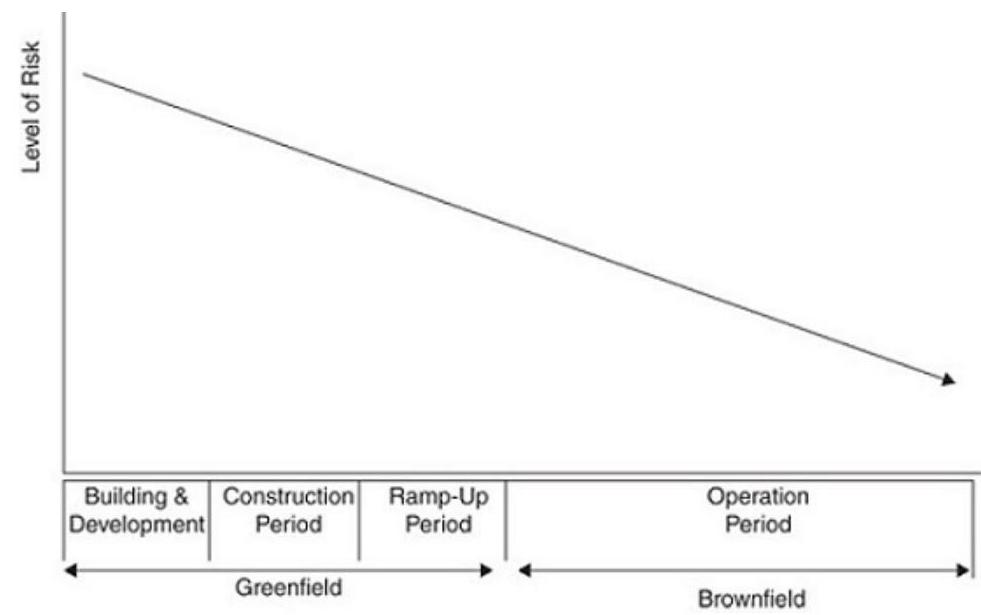
\includegraphics[max width=\textwidth]{2024_04_11_801fecba73bcef68aff8g-4}
\end{center}

Risk Profile of Infrastructure Investment Development Stages

Source: World Economic Forum (2014).

\section*{Infrastructure Investment Vehicles}
Infrastructure investments can be accessed indirectly through a number of vehicles: listed stocks, listed funds, open-end funds, and closed-end unlisted funds. Openend funds permit further investment or withdrawal of funds by investors, whereas closed-end funds have a fixed size.

Estimates of total global listed infrastructure assets vary around \$3 trillion. In 2019, the S\&P Global Infrastructure Index (S\&P GII) comprised over \$1.4 trillion of publicly traded stocks, with approximate weights of $40 \%$ utilities, $40 \%$ industrials, and $20 \%$ energy firms by asset size. Infrastructure stocks are generally regarded as having higher dividend yields and lower volatility than stocks from other sectors. The higher dividend yields can reflect, for example, the relatively inelastic demand for infrastructure services or the generally reduced growth potential for infrastructure assets compared to overall equities. The lower volatility can be attributed to the monopolistic and regulated nature of infrastructure assets, as well as the price-inelastic demand for the goods and services generated by many infrastructure assets.

Investing in listed infrastructure stocks or funds of infrastructure stocks over unlisted funds has the advantages of greater liquidity and a clearer valuation process. However, these funds have exhibited higher volatility and a greater correlation to equity markets than non-market-based valuations on unlisted infrastructure funds. Closed-end infrastructure funds are typically structured like private equity funds, have a life of typically 10 to 15 years, and draw down investor capital commitments over a stated investment period of four to five years. Management fees typically range from $1 \%$ to $2 \%$ annually, in addition to carried interest of $10 \%$ to $20 \%$ over a preferred return of $8 \%$ paid at the exit of the fund or liquidation of specific investments. The appraised prices of these unlisted funds have experienced lower volatility and lower correlation to equity markets than the market prices of listed funds. However, this may be due to the appraisal-based nature of the valuation and the illiquid nature of the fund. Also, while listed funds may use $30 \%$ to $40 \%$ leverage, unlisted funds can reach $60 \%$ to $90 \%$ leverage when financing markets allow that level of borrowing. [Due to the short track record and the private nature of unlisted funds, reliable benchmark index data have not yet been disseminated or studied.]

Unlisted open-end funds, also called evergreen funds, allow investors to subscribe to or redeem from these funds on a regular basis. This provision of liquidity works only when investor redemption demands match the underlying liquidity of the fund's assets. To fund net investor redemptions, an open-end fund must have the ability to liquidate assets, attract new investors, borrow on a line of credit, or draw down cash balances. Should the demand of investors to redeem exceed these resources, gates may form. Gates are fund restrictions on investor withdrawals. Infrastructure funds may erect gates, especially during difficult markets, requiring that investor shares be redeemed over time rather than on an as-requested basis.

Some institutional investors have chosen to invest directly in infrastructure assets, in addition to or as a substitute for investing in unlisted infrastructure funds. This method of access has become increasingly popular over the past decade, especially among the larger institutions that have built in-house teams with the experience to source, analyze, structure, negotiate, and manage infrastructure assets. Direct infrastructure ownership by institutional investors was pioneered by large Canadian and Australian pension plans.

Infrastructure investments are global in nature, with approximately equal weights in the publicly listed companies of North America, Europe, and the rest of the world. Investors in a global fund accept currency risk, as the assets, debt, and cash flows of each project are typically denominated in the currency of the country where each asset is located. Investors in these funds have a risk that the value of the currency where the asset is located might depreciate relative to the value of the currency of the home country of the investor.

The next exhibit, Types of Infrastructure Investments, provides a summary of the characteristics of investing in infrastructure using three types of approaches: unlisted direct investment, unlisted funds, and listed securities.

Types of Infrastructure Investments

\begin{center}
\begin{tabular}{|llll|}
\hline
 & Unlisted Direct Investment & Unlisted Fund & Listed Securities \\
\hline
Investment size & Very high & Moderate & Low \\
Ease of access & Difficult; takes considerable time & Moderate difficulty; takes moderate time & Easy and immediate \\
Length of investment & Long term & Long term & Flexible \\
Capacity & Limited & Moderate & High \\
Liquidity & Low & Low to medium & High \\
Leverage & Low but varies & High & Moderate \\
Fees/expenses & No fees; very high expenses & High fees; low expenses & Low fees and expenses \\
Diversification & Concentrated risk; low correlation to other assets & Medium to high; low correlation to other assets & High; high correlation to other assets \\
Control & Maximum control over assets & High level of control & Limited control \\
\end{tabular}
\end{center}

\section*{Twelve Determinants of Infrastructure}
The fundamental drivers of infrastructure performance (and risk) consist of the following 12 common attributes. Each of these 12 characteristics tends to generally provide for reduced risk, making many infrastructure assets a relatively defensive investment.

\section*{1. Inelastic demand}
Most infrastructure assets and businesses provide essential services that support the functioning of society and the economy, such as power, water, and basic transportation. The indispensable nature of most infrastructure investments results in their demand being relatively inelastic to price changes and economic downturns; their long-term growth is generally proportional to overall economic growth.

\section*{2. Monopolistic market positions}
More often than not, infrastructure assets and businesses are natural monopolies, with high barriers to entry. For example, suppose an airport is the only airport for a particular city. It may be uneconomical to build a competing airport, it may be difficult to get planning approval, and the government may explicitly promise the existing operator not to permit the development of a competing airport in the catchment area.

\section*{3. Regulated entities}
Given the monopolistic nature of such infrastructure assets, governments (or government-sponsored agencies) often regulate their activities and pricing to preclude undue monopolistic practices and extra-market returns at the expense of the consumer. As regulated entities, they are often required to sell their services at approved tariffs, which are intended to generate sufficient revenues to fund operating costs plus a certain return on capital. Gas, electric, and water utilities as well as transmission assets are examples of these regulated businesses. Their effective management necessitates specialized understanding of the applicable regulatory framework as well as technical and industry expertise to generate attractive risk-adjusted returns.

Under the right management, regulated assets may be particularly attractive investments because price regulation mitigates downside risk if costs increase. This is because prices will be allowed to increase to maintain the target return rate. Moreover, returns can still be improved by outperforming the regulator's assumptions for operating costs, capital costs, and cost of capital. On the other hand, because regulated prices tend to be more stable, they may tend to be lower than unregulated prices. In addition, while improved services resulting from capital spending can lead to higher prices in unregulated investments, such increases are less likely to occur in regulated industries. Finally, depending on the provisions of the long-term contract, regulated prices may not be allowed to rise fast enough to reflect the increased cost of operations when these costs increase faster than the overall rate of inflation.

\section*{4. Capital-intensive setup, low operating costs}
While infrastructure assets are capital intensive to set up (e.g., airports, bridges, and tunnels), once established, they generally have relatively low operating costs. This provides for strong operating margins. This attribute, combined with long projected service lives, can support high levels of leverage.

\section*{5. Low volatility of operating cash flows}
In most instances, infrastructure investment revenue streams are relatively stable and predictable, often resulting from either a captive customer base or longterm contracts, regulated pricing schedules, and limited competition or licensing. Utilities are one example. Stable cash flows can also support valueenhancing financial leverage at a more attractive cost of debt capital than similar financings undertaken by more risky assets, such as private equity buyouts.

\section*{6. Resilience to economic downturns}
Due to their essential role in the economy, infrastructure businesses, once operational, are less likely to suffer from a significant permanent decline in demand, traffic, or patronage than are businesses in other industries. They are expected to better weather downturns, with the possible exception of cases in which inappropriate capital structures have been used to finance their development (e.g., too much leverage) or when demand forecasts have been grossly inaccurate. Infrastructure investments have varying levels of sensitivity to economic conditions and business cycles.

To the degree that returns from certain infrastructure investments are not sensitive to business cycles, they will help reduce the volatility of an investor's overall performance during various stages of a business cycle. The next exhibit illustrates the general economic sensitivity of various infrastructure investments. Typically, if the cash flow of an investment is contractually fixed, the value of the investment will tend to be less sensitive to changes in economic conditions.

\begin{center}
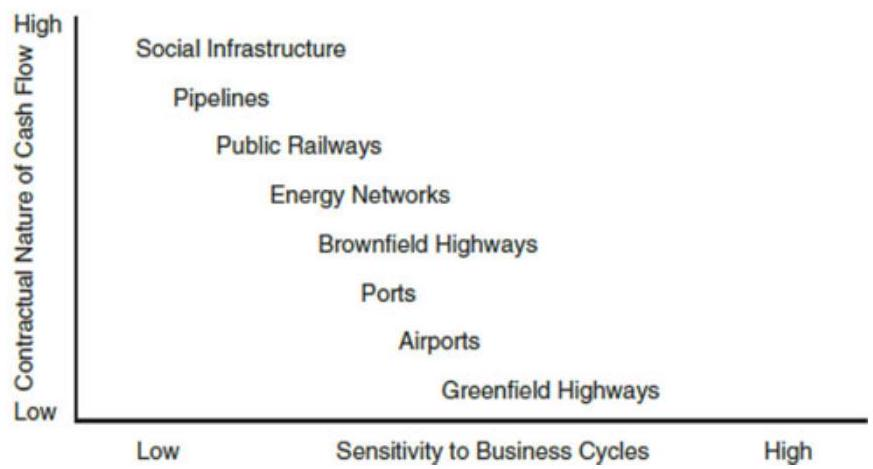
\includegraphics[max width=\textwidth]{2024_04_11_801fecba73bcef68aff8g-6}
\end{center}

Sensitivity to Business Cycles

\section*{7. Technology risk}
Many infrastructure assets are less exposed to technology obsolescence risk. However, for greenfield infrastructure that is reliant on technology (e.g., power generation), it is important to ensure that the technology used is proven or that the risk of technology failure is otherwise mitigated.

\section*{8. Long-term horizons}
Infrastructure assets have long and useful economic lives (often over 50 years), producing stable revenues with relatively stable cash flows. This long-term predictability may be helpful to investors seeking to match long-term yielding assets against long-term liabilities (e.g., pension plan and insurance company liabilities).

\section*{9. Inflation-indexed cash flows}
Infrastructure assets may have contractual or regulatory revenue structures that are adjusted for changes in measures of inflation, such as the Consumer Price Index, thus making for an effective inflation hedge. Their long-term inflation-linked cash flow characteristics are attractive duration hedges for long-term liabilities. Foreign infrastructure investment projects expose investors to currency fluctuations. If cash flows are contractually fixed, this will make future cash flows more predictable and may reduce the cost of financing these projects. However, the real value of the cash flows will suffer if there is an unexpected increase in inflation. To the degree that the local currency may depreciate in response to higher inflation, foreign investors will see the value of the cash flows converted into their own currency decline as well.

\section*{10. Stable yield}
A consequence of the low operating costs and stable revenues is the ability of mature infrastructure businesses to support relatively high dividend yields, typically in the mid-to-high single digits per annum, in conjunction with moderate capital appreciation. This contrasts with private equity or venture capital investments, which are focused on capital growth for the great majority of the investment return.

\section*{11. Low correlation with other asset classes}
Infrastructure businesses typically display low correlation with traditional asset classes. One reason for this apparent low correlation is that valuation may be appraisal-based, which leads to smoothed returns. When returns are smoothed, their volatilities are artificially reduced and their correlations with traditional asset classes are moved toward zero. The other reason is that infrastructure businesses are regulated and have inelastic demand, leading to stable cash flows. Therefore, while infrastructure investments are expected to provide significant diversification benefits when added to a portfolio consisting of traditional asset classes, empirical estimates of these benefits could be overstated.

\begin{enumerate}
  \setcounter{enumi}{11}
  \item Potentially low total and idiosyncratic risks
\end{enumerate}

Many infrastructure investments have relatively low idiosyncratic risks. Total historical average returns from mature infrastructure investments have tended to depend on various factors, including the sector and jurisdiction in which the business operates. For example, with exceptions, a mature regulated gas utility has tended to have low idiosyncratic risks and to provide a lower return to investors (due to the lower risk as a result of the regulated nature of the business and the reliability of future cash flows). Returns from investments in sectors such as airports and ports (in part due to the variability of revenue as a result of exogenous factors) tend to have higher volatility.

\section*{Opportunities and Allocations in Infrastructure Investments}
Infrastructure has traditionally been under the purview of governmental bodies. Its importance from a public interest perspective cannot be overstated. For several reasons, there has been globally widespread historical underinvestment, resulting in degradation of existing assets with a simultaneous failure to add sufficient new capacity. As this issue is unlikely to reverse course any time soon, forward-thinking countries and government entities have sought to encourage the convergence of public and private sector activity. Their aim is to help the creation of economically viable new infrastructure assets and upgrade, properly maintain, manage, and operate existing ones. Formal contracting structures through active PPPs supported by recent government initiatives have made progress in encouraging private capital investment in infrastructure. However, there remains a lot to be done.

The market opportunities in developed countries remain substantial. These opportunities are in civil aviation, bridges, roads, mass transit, railways, greenfield and brownfield projects, dams, water, waste management, and energy. The success of many new fund launches exclusively dedicated to infrastructure investing is suggestive of the vital role that private finance will continue to play in infrastructure development. This overall positive sentiment notwithstanding, many institutional investors have yet to ramp up their investment capabilities in this area. Some of them have not made dedicated allocations to infrastructure, perhaps reflecting the relative infancy of this asset class. Consequently, possibilities for early-mover advantages may remain in developed countries and are arguably even higher elsewhere. Government policy, changing legislation and regulatory norms, and private capital flows will strongly influence the evolution of infrastructure investments.

There is a debate about where infrastructure fits in an investor's asset allocation, as infrastructure has commonalities with fixed-income (institutional bonds), institutional real estate, and private equity investments. The exhibit below summarizes the four investments across seven characteristics. Some investors consider infrastructure as a fixed-income investment due to its high current yield, steady cash flows, and long duration. Infrastructure is similar to real estate and physical assets in terms of generating cash flows. Social infrastructure may have more in common with real estate investments than energy or utility infrastructure. Investors considering infrastructure as a private equity investment focus on the control aspect of infrastructure operating companies and the ability to add value through financial engineering or operating improvements. A CFA Institute paper estimates that $34 \%$ of investors consider infrastructure as part of their private equity allocation, $16 \%$ place it in the real estate or real assets allocation, and $50 \%$ consider it a unique asset class.

Characteristics Associated with Infrastructure and Other Asset Categories

\begin{center}
\begin{tabular}{|c|c|c|c|c|}
\hline
 & Infrastructure & Institutional Bonds & Institutional Real Estate & Private Equity \\
\hline
Nature of asset & \begin{tabular}{l}
Typically an operating company dependent \\
on control of large, physical assets \\
\end{tabular} & Financial security & Physical property & Operating company \\
\hline
Asset availability & \begin{tabular}{l}
Asset scarcity; many in unique, monopoly \\
situations \\
\end{tabular} & \begin{tabular}{l}
Deep volumes in \\
most markets \\
\end{tabular} & \begin{tabular}{l}
Moderate to deep volumes \\
in most markets \\
\end{tabular} & Moderate volumes in most markets \\
\hline
Acquisition dynamic & \begin{tabular}{l}
Competitive tenders; regulatory, \\
environmental, social, and political issues; \\
often held for the long run \\
\end{tabular} & \begin{tabular}{l}
Efficient, on-market \\
purchase \\
\end{tabular} & \begin{tabular}{l}
Competitive tenders; \\
environmental and social \\
issues common \\
\end{tabular} & \begin{tabular}{l}
Competitive tenders, management \\
buyout, negotiated trade sale, typically \\
medium-term exit strategy \\
\end{tabular} \\
\hline
Liquidity & Moderate & Very high & Moderate in most sectors & Moderate \\
\hline
Income & \begin{tabular}{l}
Once assets mature, very stable; \\
inflation/GDP growth relative; typically \\
higher than bonds and core real estate \\
\end{tabular} & \begin{tabular}{l}
Fixed coupon; \\
sensitive to interest \\
rates \\
\end{tabular} & \begin{tabular}{l}
Mixture of fixed and variable \\
interest rates and sector \\
dependent \\
\end{tabular} & Typically dominated by capital returns \\
\hline
Growth & \begin{tabular}{l}
Dependent on asset stage; modest (late \\
stage) to high (early stage/development \\
assets) \\
\end{tabular} & Low & \begin{tabular}{l}
Dependent on asset \\
characteristics; moderate to \\
high \\
\end{tabular} & \begin{tabular}{l}
Dependent on asset characteristics; \\
typically high \\
\end{tabular} \\
\hline
Volatility & Moderate (early stage) to low (late stage) & \begin{tabular}{l}
Moderate (market \\
factors) \\
\end{tabular} & Low/moderate & \begin{tabular}{l}
High (early stage) to moderate (late \\
stage) depending on industry sector \\
\end{tabular} \\
\hline
\begin{tabular}{l}
Typical return \\
expectation per \\
annum post fees \\
\end{tabular} & \begin{tabular}{l}
Mature portfolio: $7 \%-10 \%$; development \\
portfolio: > 10\% \\
\end{tabular} & \begin{tabular}{l}
Approximately $5 \%-$ \\
$7 \%$ \\
\end{tabular} & \begin{tabular}{l}
Core: $\sim 7 \%-9 \% ;$ value added: \\
$\sim 12 \%-18 \% ;$ opportunistic: > \\
$18 \%$ \\
\end{tabular} & Diversified portfolio: > 15\% \\
\hline
\end{tabular}
\end{center}

Source: Data from "Understanding Infrastructure," RREEF, 2005.

From an alternative investment perspective, infrastructure assets exhibit different risk-return profiles from other private investments; they can be a source of alpha as well as a valuable diversification tool in portfolio construction. They provide exposure through both illiquid long-term private vehicles and liquid publicly traded funds. This versatility makes them attractive for various investor segments.


\end{document}